\section{Vorarbeit}
Im Projekt2 \citetitle{project2} \cite{project2} wurde eine Datensammlung von vier deutschschweizer Online-Medien erstellt von Artikeln welche in den letzten 22 Jahren veröffentlicht wurden.
Bestandteil dieser Arbeit war, einen spezifischen Webcrawler pro Nachrichtenportal zu bauen und automatisiert über einen GitLab Job Scheduler (vgl. Kapitel \ref{gitlab}) laufen zu lassen.
Der gesammelte Datensatz umfasst mit über 300'000 Artikeln (Stand vom Januar 2023) aus vier der fünf grössten frei zugänglichen Nachrichtenportalen \cite{statista-nachrichtenportale-marktanteil}
der Deutschschweiz einen bedeutenden Teil der online zugänglichen Zeitungsartikel, welche die hiesige Bevölkerung in den letzten Jahren
gelesen hat. In der Abbildung \ref{p2-count-articles} ist ersichtlich, wie viele Artikel wir am Ende von Projekt2 pro Nachrichtenportal gesammelt haben.
Die Artikel von Blick, Watson, SRF und 20 Minuten sind in einer MongoDB Datenbank auf einer virtuellen Maschine der BFH gespeichert.
In dieser Bachelor Thesis dient dieser Datensatz als Grundlage für die Analyse des Gender Gaps in den deutschschweizer Online-Medien.

\begin{figure}[H]
	\begin{center}
        \centering
		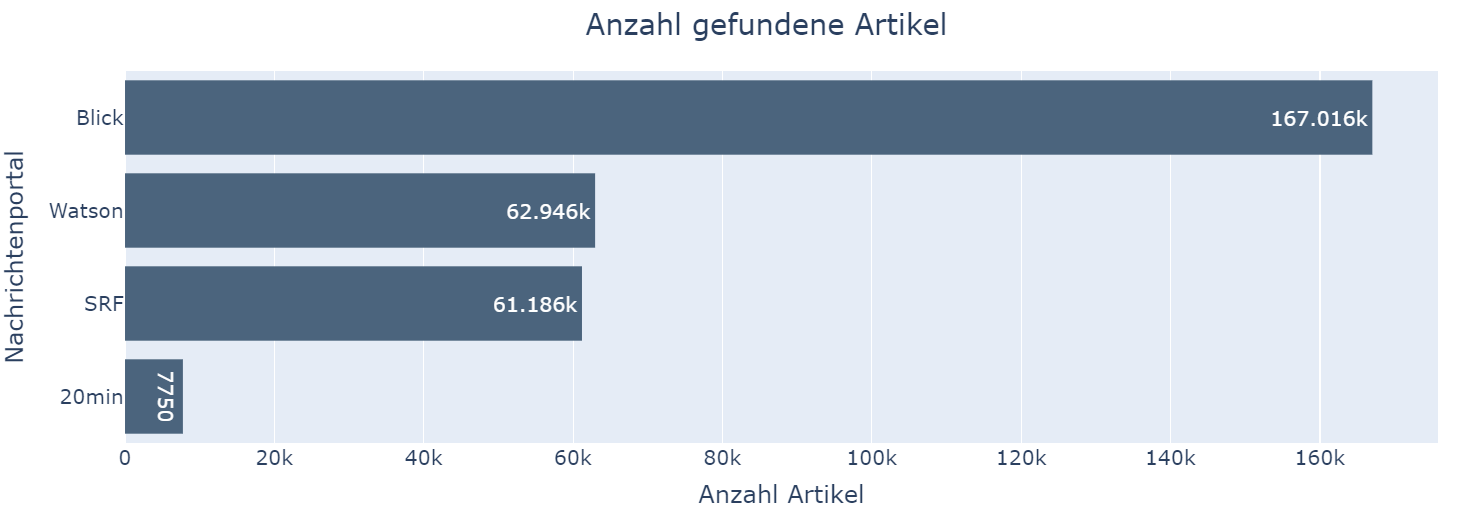
\includegraphics[width=1\linewidth]{./images/sum_all_2015-20230102.png}
		\caption{Anzahl Artikel pro Nachrichtenportal (unbereinigt), Stand 02.01.2023}
		\label{p2-count-articles}
	\end{center}
\end{figure}

Als Vorbereitung für die vorliegende Arbeit wurde eine grobe Methodik für das Extrahieren der Zitate, 
Personen und der geschlechtsbezogenen Informationen definiert. 
Die Methodik wurde inspiriert von der wissenschaftlichen Arbeit \citetitle{gender_gap_tracker} \cite{gender_gap_tracker}, 
welche auch die Grundinspiration dieser Bachelor Thesis ist.
